\chapter{Конструкторский раздел}

В этом разделе будет представлено описание используемых типов данных, а также схематические изображения алгоритмов сортировок: блочной, быстрой и выбором.

\section{Требования к программному обеспечению}

Программа должна поддерживать два режима работы: режим массового замера времени и режим сортировки введенного массива.

Режим массового замера времени должен обладать следующей функциональностью:
\begin{itemize}
	\item генерировать массивы различного размер для проведения замеров;
	\item осуществлять массовый замер, используя сгенерированные данные;
	\item результаты массового замера должны быть представлены в виде таблицы и графика.
\end{itemize}

К режиму сортировки выдвигается следующий ряд требований:
\begin{itemize}
	\item возможность работать с массивами разного размера, которые вводит пользователь;
	\item наличие интерфейса для выбора действий;
	\item на выходе программы массив, отсортированный тремя алгоритмами по возрастанию.
\end{itemize}

\section{Описание используемых типов данных}

При реализации алгоритмов будут использованы следующие структуры и типы данных:
\begin{itemize}
	\item целое число представляет количество элементов в массиве;
	\item список целых чисел;
\end{itemize}

\section{Разработка алгоритмов}

На рисунке \ref{pic:blocksort} приведена схема алгоритма блочной сортировки.

\begin{figure}[H]
	\centering
	
\includegraphics[scale=0.5]{assets/blocksort.pdf}
	\caption{Схема алгоритма блочной сортировки}
	\label{pic:blocksort}
\end{figure}

\newpage

На рисунке \ref{pic:quicksort} приведена схема алгоритма быстрой сортировки.

\begin{figure}[H]
	\centering
	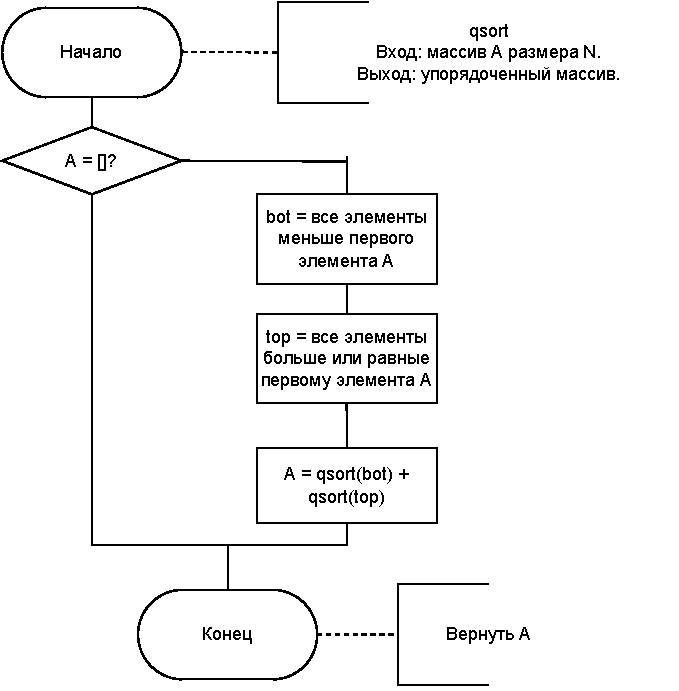
\includegraphics[scale=1]{assets/quicksort.pdf}
	\caption{Схема алгоритма быстрой сортировки}
	\label{pic:quicksort}
\end{figure}

\newpage

На рисунке \ref{pic:selectionsort} приведена схема алгоритма сортировки выбором.

\begin{figure}[H]
	\centering
	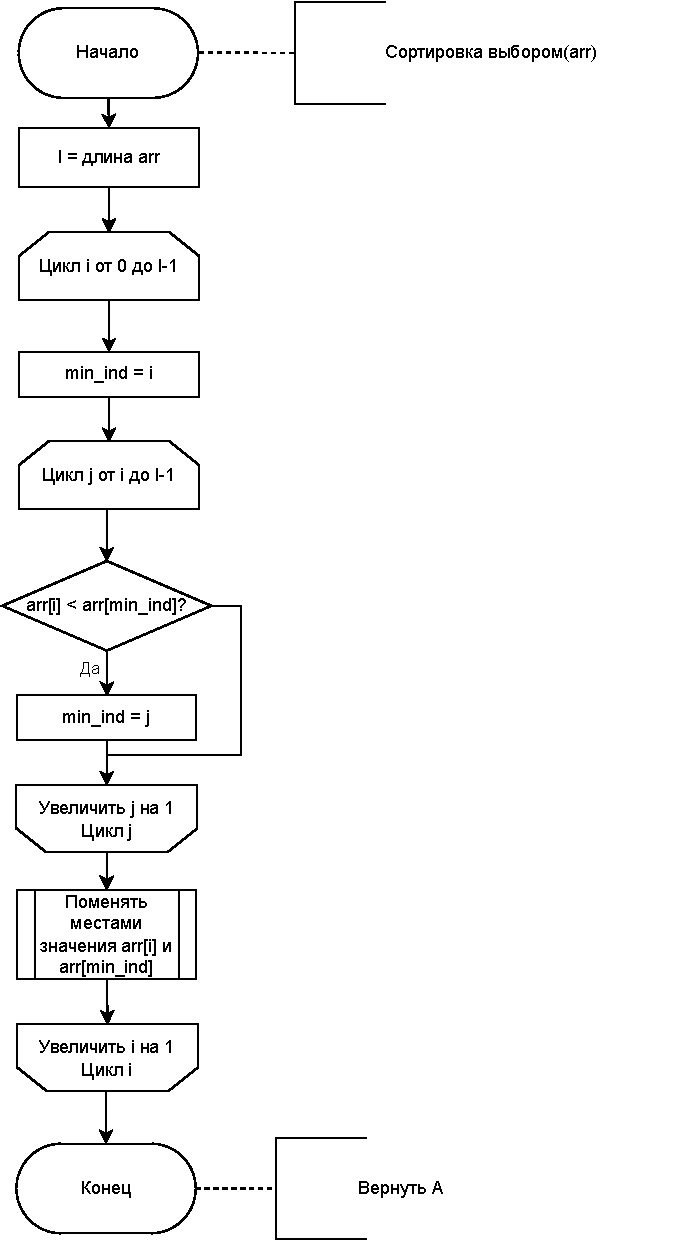
\includegraphics[scale=1]{assets/selectionsort.pdf}
	\caption{Схема алгоритма сортировки выбором}
	\label{pic:selectionsort}
\end{figure}

\newpage


\section{Оценка трудоемкости алгоритмов}

Модель для оценки трудоемкости алгоритмов состоит из шести пунктов:
\begin{enumerate}
	\item $+, -, =, +=, -=, ==, ||, \&\&, <, >, <=, >=, <<, >>, []$ --- считается, что эти операции обладают трудоемкостью в 1 единицу;
	\item $*, /, *=, /=, \% $ --- считается, что эти операции обладают трудоемкостью в 2 единицы;
	\item трудоемкость условного перехода принимается за $0$;
	\item трудоемкость условного оператора рассчитывается по следующей формуле
	\begin{equation}
		\label{eq:if}
		f_{if} = f_{\text{условия}} + 
		\begin{cases}
			min(f_1, f_2), & \text{лучший случай}\\
			max(f_1, f_2), & \text{худший случай}
		\end{cases},
	\end{equation}
	где $f_1$ --- трудоемкость блока, который вычисляется при выполнении условия, а $f_2$ --- трудоемкость блока, который вычисляется при невыполнении условия;
	\item трудоемкость цикла рассчитывается по следующей формуле
	\begin{equation}
		\label{eq:for}
		\begin{gathered}
			f_{for} = f_{\text{инициализация}} + f_{\text{сравнения}} + M_{\text{итераций}} \cdot (f_{\text{тело}} +\\
			+ f_{\text{инкремент}} + f_{\text{сравнения}});
		\end{gathered}
	\end{equation}
	\item вызов подпрограмм и передача параметров принимается за $0$.
\end{enumerate}

\subsection{Трудоемкость алгоритма блочной сортировки}

В данной реализации размер блока обозначается как $k$, трудоемкость операции добавления и удаления элемента из вектора равна 2.


\textbf{Лучший случай:} массив отсортирован, элементы распределены равномерно (все блоки содержат одинаковое число элементов), расчет трудоемкости данного случая приведен в следующей формуле

\begin{equation}
	\label{сomplexity:block_best}
	\begin{gathered}
		f_{best} = 1 +1 + \frac{n}{k} \cdot(1 + 2+f_{shaker} + 2 + 1 + 4 + \\
		+ k \cdot (3 + 1 + 4)) + 1 + 1 + \\
		+ \frac{n}{k} \cdot (1 + 4 + 1 + 1 + 5 + 1 + 4 + 1 + 1 + n \cdot (5)) = \\
		= 4 + \frac{29\cdot n + n \cdot f_{shaker} + 5 \cdot n^2}{k}  + 8 \cdot n  = \\
		= 4 + 8 \cdot n + 29 \cdot \frac{n}{k} + n \cdot (14.5 + \frac{k}{2}) + \frac{5 \cdot n^2}{k} = \\
		= 4 + 8 \cdot n + 29 \cdot \frac{n}{k} + 14.5 \cdot n + \frac{n \cdot k}{2} + \frac{5 \cdot n^2}{k} = \\
		= \frac{5 \cdot n^2}{k} + 22.5 \cdot n + 29 \cdot \frac{n}{k} + \frac{n \cdot k}{2} + 4.
	\end{gathered}
\end{equation}

\textbf{Худший случай:} большое количество пустых блоков, массив отсортирован в обратном порядке (худший случай сортировки перемешиванием, которая используется в блочной сортировке), расчет трудоемкости приведен в следующей формуле

\begin{equation}
	\label{сomplexity:block_worst}
	\begin{gathered}
		f_{worst} = 1 +1 + \frac{n}{k} \cdot(1 + 2+f_{shaker} + 2 + 1 + 4 + \\
		+ k \cdot (3 + 1 + 4)) + 1 + 1 + \\
		 + \frac{n}{k} \cdot (1 + 4 + 1 + 1 + 5 + 1 + 4 + 1 + 1 + k \cdot (6)) = \\
		= 4 + \frac{29\cdot n + n \cdot f_{shaker} + 6 \cdot n^2}{k}  + 8 \cdot n  = \\
		= 4 + 8 \cdot n + 29 \cdot \frac{n}{k} + n \cdot (19.5 + \frac{k}{2}) + \frac{6 \cdot n^2}{k} = \\
		= 4 + 8 \cdot n + 29 \cdot \frac{n}{k} + 19.5 \cdot n + \frac{n \cdot k}{2} + \frac{6 \cdot n^2}{k} = \\
		= \frac{6 \cdot n^2}{k} + 27.5 \cdot n + 29 \cdot \frac{n}{k} + \frac{n \cdot k}{2} + 4.
	\end{gathered}
\end{equation}


\subsection{Трудоемкость алгоритма быстрой сортировки}

Чтобы вычислить трудоемкость алгоритма быстрой сортировки, нужно учесть следующее:

\begin{enumerate}[label=---]
		
	\item трудоемкость уcловного оператора на проверку $pivot$ в теле цикла вычисляется по следующей формуле
	
	\begin{equation}
	\label{eq:2.1}
	f_{if\_pivot} = 1 + 
	\begin{cases}
	2 + 1, \\
	0
	\end{cases}
	\end{equation}		

	\item трудоемкость цикла, в теле которого уcловный оператор на проверку $pivot$, вычисляется по следующей формуле

	\begin{equation}
	\label{eq:2.2}
	f_{for\_low\_high} = 1 + M \cdot f_{if\_pivot}
	\end{equation}

	\item трудоемкость уcловного оператора на проверку $low$ в теле цикла вычисляется по следующей формуле

	\begin{equation}
	\label{eq:2.2}
	f_{if\_low
	} = 1 + 
	\begin{cases}
	1, \\
	0
	\end{cases}
	\end{equation}		

	\item трудоемкость цикла, в теле оператор ветвления $f_{if\_low}$ и $f_{for\_low\_high}$, вычисляется по следующей формуле

	\begin{equation}
	\label{eq:2.3}
	f_{while\_stack} = 1 + N \cdot (2 + f_{if\_low} + 2 + f_{for\_low\_high}
	+ 2 + 2)
	\end{equation}
	
	\item трудоемкость уcловного оператора на проверку длины массива вычисляется по формуле
	
	\begin{equation}
	\label{eq:2.4}
	f_{if\_len} = 1 + 
	\begin{cases}
	1, \\
	1 + f_{while\_stack}
	\end{cases}
	\end{equation}	
		
\end{enumerate}
		
В итоге, трудоемкость быстрой сортировки вычисляется по формуле
\begin{multline}
\label{eq:2.5}
f_{quick\_sort} = 1 + f_{if\_len} = 1 + 1 + N \cdot (2 + f_{if\_low} + 2 + f_{for\_low\_high}) = \\
1 + 1 + N \cdot (2 + 2 + 2 + 1 + M \cdot f_{if\_pivot} + 2 + 2) = \\
1 + 1 + N \cdot (2 + 2 + 2 + 1 + M \cdot (3 + 2 + 2) + 1 + 3 + 2 + 1 = \\
2 + 7N + 7MN +7N = 14N + 7MN 
\end{multline}

\subsection{Трудоемкость алгоритма сортировки выбором}

Трудоемкость сортировки выбором в худшем случае $O(N^2)$.

Трудоемкость сортировки выбором в лучшем случае $O(N^2)$.

Худший и лучший случаи совпадают~\cite{selectionsort}.


\section*{Вывод}
На основе теоретических данных, полученных из аналитического раздела были построены схемы требуемых алгоритмов. 
Была введена модель оценки трудоемкости алгоритма, были рассчитаны трудоемкости алгоритмов в соответствии с этой моделью.

В результате теоретической оценки трудоемкостей алгоритмов выяснилось, что лучшей асимптотической оценкой во всех случаях обладает быстрая сортировка.
Худшей асимптотической оценкой во всех случаях обладает сортировка выбором $O(N^2)$.